%\section{Rules of Differentiation}
\vspace{-0.25 in}
\begin{framed}
\subsection*{Objectives}
\begin{itemize}
    \item Be familiar with some of the basic rules for finding derivatives of functions
    \item Understand how the derivative of a function is used to determine the slope of the graph of the function at a point
    \item Understand the interpretation and use of the derivative in \textbf{marginal analysis} (business and economics).
\end{itemize}

%%%Reading Assignment%%%
\subsection*{Suggested Reading:}
\begin{itemize}
\item \cite{Calaway}\footnotemark[1]
   \begin{itemize}
        \item \emph{Section 2.3 Power and Sum Rules for Derivatives}
        \begin{itemize}
            \item Disregard the derivatives for \emph{Exponential Functions} and \emph{Natural Logarithm}. We will discuss about these rules in the future lessons.
            \item Skip \emph{Example 7}
        \end{itemize}
    \end{itemize}

\item \cite{openstaxColAlgebra}\footnotemark[2]
    \begin{itemize}
        \item Review rules of exponents; exponents and rational exponents from \emph{sections 1.2-1.3 }.
        
    \end{itemize}

\end{itemize}
%\subsection*{Supplemental Materials:}
%%%Key Terms%%%
\subsection*{Key Terms and Concepts:} 

\begin{multicols}{2}
\begin{itemize}
    \item Rules for finding derivatives of functions
    \item Notation for derivatives of functions
    \item Slope of a graph at a point
    \item Equation of a tangent line
    \item Marginal cost, Marginal profit and Marginal revenue
\end{itemize}
\end{multicols}
\end{framed}
\footnotetext[1]{Available free to download from \url{http://www.opentextbookstore.com/details.php?id=14} .}
\footnotetext[2]{Available free to download from \url{https://openstax.org/details/books/college-algebra} .}

\newpage
%%%%%%%%%%START LESSON CONTENT%%%%%%%%%%%%%
%\noindent\makebox[\linewidth]{\rule{\textwidth}{0.8pt}}

%%%%%%%%%%%%%%%%Start First Topic%%%%%%%%%%%%%%%%%%%%%%%%%%%%%
\section*{Using Basic Differentiation Rules}


\noindent A formula for the derivative function (see equation \ref{eq:dervLimit} in lesson \ref{introDerv}) is very powerful, but as you can see, calculating the derivative using the limit definition is very time consuming. In this section, we will use some simple rules\footnotemark for finding derivatives of basic functions without needing the limit definition. In the following lessons, we will consider some additional rules for differentiation that will allow us to find derivatives for more complicated functions.\\
\noindent Recall that in section \ref{introDerv} the alternative notations for the derivative were introduced using \(\displaystyle\frac{d}{dx}f(x)\) and \(\displaystyle\frac{dy}{dx}\) (read as \emph{“the derivative of y with respect to x”.}). You will want to be familiar and comfortable with these various notations since they will be used when the rules are provided in this section.
\footnotetext{To make sense out of these rules, see \emph{Building Blocks} (examples 1-3) in section 2.3 from \cite{Calaway}.}
%%%%%%%%%%%%%Basic Differentiation Rules%%%%%%%%%%%
\begin{tcolorbox}[title = {Differentiation Rules: Basic Rules}]

\noindent In what follows, $f(x)$ and $g(x)$ are differentiable functions of $x$ and $k$ is a constant.\\

\textbf{Constant Multiple Rule:}
\begin{equation}\label{eq:constantMultiple}
\frac{d}{dx}(kf(x))=kf'(x)
\end{equation}

\textbf{Sum Rule:}
\begin{equation}\label{eq:SumRule}
\frac{d}{dx}(f(x)+g(x))=f'(x)+g'(x)
\end{equation}

\textbf{Difference Rule:}
\begin{equation}\label{eq:DiffRule}
\frac{d}{dx}(f(x)-g(x))=f'(x)-g'(x)
\end{equation}

\textbf{Power Rule:}
\begin{equation}\label{eq:PowerRule}
\frac{d}{dx}(x^n)=nx^{n-1}
\end{equation}

\textbf{Constant Rule:}\footnotemark
\begin{equation}\label{eq:ConstantRule}
\frac{d}{dx}(k)=0
\end{equation}

\end{tcolorbox}
\footnotetext{The derivative of a constant is zero because \(k=kx^0\).}
%%%%%%%%%%%%%%%%%%%%%%%%%%%%%%%%%%%%%%
\Opensolutionfile{ans}[ans4]
\Opensolutionfile{ansL}[ansL4]

\noindent Examples \ref{exBasicRules1}-\ref{exBasicRules3} show that the sum, difference, and constant multiple rule combined with the power rule allow us to easily find the derivative of a function. However, converting the math expressions into exponents is needed before taking the derivative using the \emph{Power Rule} in the equation \ref{eq:PowerRule}.The review of some \emph{Rules of Exponents}\footnotemark that are useful when translating a math expression into exponents is shown on page \pageref{eq:quotientRuleExp}.

\footnotetext{See sections 1.2-1.3 from \cite{openstaxColAlgebra} for full review on \emph{Exponents and Rational Exponents}. For the online version, visit \url{https://openstax.org/details/books/college-algebra}}
\newpage

%%%%%%%%%Rule of Exponents%%%%%%%%%%%%%
\begin{tcolorbox}[title = {Review: Some Rules of Exponents}]

\textbf{The Negative Rule of Exponents:}
\noindent For any real number $a$ and natural numbers $n$, the negative rule of exponents states that 
\begin{equation}\label{eq:negativeRuleExp}
\frac{1}{a^n}=a^{-n}
\end{equation}

\textbf{Rational Exponents:}
\noindent Rational exponents are another way to express principal $n$th roots. The general form for converting between a radical expression with a radical symbol and one with a rational exponent is
\begin{equation}\label{eq:rationalExp}
\sqrt[n]{a^m}=a^{\frac{m}{n}}
\end{equation}

\textbf{The Quotient Rule of Exponents:}
\noindent For any real number $a$ and natural numbers $m$ and $n$, such that $m>n$,  the quotient rule of exponents states that 
\begin{equation}\label{eq:quotientRuleExp}
\frac{a^m}{a^n}=a^{m-n}
\end{equation}


\textbf{The Product Rule of Exponents:}
\noindent For any real number $a$ and natural numbers $m$ and $n$, the product rule of exponents states that 
\begin{equation}\label{eq:productRuleExp}
a^m\cdot a^n=a^{m+n}
\end{equation}

\textbf{The Power Rule of Exponents:}
\noindent For any real number $a$ and natural numbers $m$ and $n$, the power rule of exponents states that 
\begin{equation}\label{eq:powerRuleExp}
(a^m)^n=a^{m\cdot n}
\end{equation}

\end{tcolorbox}
%%%%%%%%%%%%%%%%%%%%%%%%%%%%%%%%%%%%%%%%%%%%%%%%

%%%Examples%%%
%ex1 from Dave's handout 1.6 Rules for Differentiation (Sp2020)
\begin{example}\label{exBasicRules1}
Given $y=\displaystyle \frac{2}{x^2}$, find $\displaystyle\frac{dy}{dx}$.
    %%short answer
    \begin{sol}
    $\displaystyle\frac{dy}{dx}=-\frac{4}{x^3}$
    \end{sol}
    %%solution
    \begin{solL}
    Complete solution here.....
    
    \end{solL}
    
\end{example}
\vspace{1in}
%%%%%%%%%%%%%%%%%%%%%%%%
%%%Examples%%%
%MyOpenMath > Business Calculus by Calaway > 2.5 Derivatives Formulas > Question 12 > Question ID: 16126
\begin{example}\label{exBasicRules2}
Given $f(x)=\displaystyle\frac{3x^5-4x^4-6x^3}{x^4}$, find $f'(x)$.
    %%short answer
    \begin{sol}
    $f'(x)=3+\displaystyle\frac{6}{x^2}$
    \end{sol}
    %%solution
    \begin{solL}
    Complete solution here.....
    
    \end{solL}
    
\end{example}
\vspace{1.2in}
%%%%%%%%%%%%%%%%%%%%%%%%
%%%Examples%%%
%ex2 from Dave's handout 1.6 Rules for Differentiation (Sp2020)
\begin{example}\label{exBasicRules3}
Given $f(x)=2\sqrt{x}+3x$, find $f'(x)$. Then, evaluate $f'(1)$
    %%short answer
    \begin{sol}
    $f'(x)=\displaystyle\frac{1}{\sqrt{x}}+3$ ; 3
    \end{sol}
    %%solution
    \begin{solL}
    Complete solution here.....
    
    \end{solL}
    
\end{example}
\newpage
\section*{Finding the Equation of a Tangent Line}
In section \ref{introDerv}, we first discussed about the derivative as the slope of the line tangent to a graph. We will revisit this concept again with using the basic differentiation rules instead of using limits.
%%%%%%%%%%%%%%%%%%%%%%%%
%%%%Optional: From OpenStax Calculus I, ex3.22;pg.252.

%%%%Last Question from Dave's 1.6 Rules for Differentiation
\begin{example}
Given $f(x)=\displaystyle\frac{3}{x^2}+x$,
\renewcommand{\labelenumi}{(\arabic{enumi})}
\begin{enumerate}[leftmargin=*]
\item Using the differentiation rule(s), find $f'(x)$ .
\item Using the derivative of $f$, find the slope of the line tangent to the graph of $f$ at the point $(-1,2)$.
\item Find the equation of the line tangent to the graph of $f$. Use the point-slope form: $y=mx+b$.
\label{eqTangExC}
\end{enumerate}

\vspace{-0.5cm}
\begin{figure}[H]
  \hspace*{-9cm}
    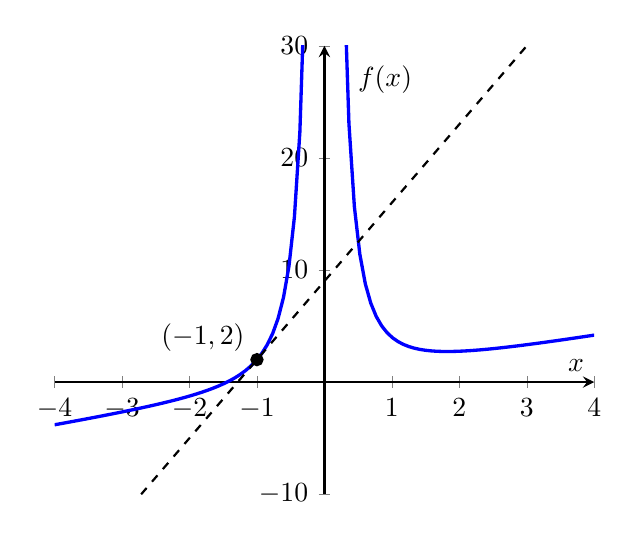
\begin{tikzpicture}[scale=1]
        \begin{axis}[ xlabel={$x$},axis lines=middle,xtick={-4,...,4},samples=100, thick,domain=-4:4,ymin=-10,ymax=30]
            \addplot+[no marks,very thick] {3/x^2 +x};
             \node at (axis cs:0.9,27) {$f(x)$};
             \addplot [color=black,mark=*,mark size=2pt] coordinates {(-1,2)};
            \node at (axis cs:-1.8,4) {$(-1,2)$};
            \addplot+[no marks,color=black,dashed, thick]{(7*x+9};
        
        \end{axis}
    \end{tikzpicture}
    \captionsetup{justification=justified,singlelinecheck=off }
        
    \caption{Graphing can verify the line found \\in part
          (\ref{eqTangExC}) is indeed tangent to the graph of $f$.}
    \label{fig:eqTangEx}
\end{figure}
    %%short answer
    \begin{sol}
    (1) $f'(x)=\displaystyle\frac{-6}{x^3}+1$ (2) $m=7$ (3) $y=7x+9$
    \end{sol}
    %%solution
    \begin{solL}
    ???
    
    \end{solL}
    
\end{example}
\vspace{0.4in}
%%%%%%%%%%%%%%Example%%%%%%%%%%%%%%%%%%%%%%%%%
%%%%%%%Question 8 from MyOpenMath>Business Calculus by Calaway> Assignment 2.5 Derivatives of Formulas
\begin{example}\label{exHorzTang}

Given $f(x)=2x^3+6x^2-144x+18$, find $f'(x)$ \textbf{using the differentiation rules.} Then determine \textbf{all points} for which the \underline{slope of the tangent line is zero} (horizontal line). Use a graphing calculator to verify your answers by graphing the function $f$ and determine if the lines tangent to these points are actually zeros.\footnotemark
    %%short answer
    \begin{sol}
    (-6,666) and (4,-334)
    \end{sol}
    %%solution
    \begin{solL}
    Complete solution here.....
    
    \end{solL}
    
\end{example}

\footnotetext{\textbf{Desmos} online graphing calculator or \textbf{Geogebra} online graphing calculator are strongly recommended. They are available online for free from \url{https://www.desmos.com/calculator} and \url{https://www.geogebra.org/graphing?lang=en}. You may also download their apps on your smartphone for free. }

\footnotetext{To graph the function in Desmos graphing calculator, type $f(x)=2x^3+6x^2-144x+18$ and then click the wrench icon on the top right to adjust the x-axis and y-axis settings. Change the default settings to $-15\le x \le 15$ and $-4000\le y \le 4000$. You may find the following tutorial videos helpful for basic graphing in Desmos: \url{https://youtu.be/7oVOs9TX57s} and \url{https://youtu.be/En_PkyA-4_4} }
%%%%%%%%%%%%End Examples%%%%%%%%%%%%%%%%%%
%%%%%%%%%%%%%%%End Topic%%%%%%%%%%%%%%%%%%
%%%%%%%%%%%%%%%%Begin Next Topic%%%%%%%%%%%%%%%%%%%%%%%%%%%%%%%
\newpage
\vspace{-1cm}
\section*{Marginal Analysis}
In economics, production processes are often analyzed by using cost ($C$), revenue ($R$), and profit ($P$) functions.  Each function uses the production level, $x$, as the independent variable.  A question of interest is finding the approximate additional cost, revenue, or profit that results when the production level is increased by one unit above the current level.  From the previous result, we can \textbf{approximate} (or \textbf{predict}) the change in these functions by using their derivatives .  For example, $C'(a)$ is used to approximate the change in total cost when the production level is increased from $x=a$ to $x=a+1$: $C'(a)\approx C(a+1)-C(a)$.  In this context, $C'(a)$ is called the “marginal cost at production level a”, or the "\textbf{marginal cost} of producing a units”.  It is interpreted as the \textbf{additional cost} of the \emph{“next unit”} of production.  Similar interpretations are given to $R'(a)$ and $P'(a)$.  In general, the marginal cost, revenue, and profit functions are denoted by $C'(a)$, $R'(a)$, and $P'(a)$.
%%%Examples%%%
%%%%%%From Dave, 1.7 More on Derivatives Handout
\begin{example}
Suppose a manufacturer has determined that the monthly profit associated with producing $x$ gallons of pesticide may be modeled by the function $P(x)=-.01x^2+6x-100$ dollars, $x\ge 0$.
\renewcommand{\labelenumi}{(\arabic{enumi})}
\begin{enumerate}[leftmargin=*]
\item Find the marginal profit function.\vspace{1in}
\item Find the marginal profit when production is $x=100$ gallons and interpret the result.  Compare this \textbf{approximate} change in profit to the \textbf{actual} change when increasing production from 100 to 101 gallons. \vspace{2in}
\item Using the concept of \textbf{marginal analysis}, by how much would you \textbf{predict} the profit will change if the  production is increased from $x=400$ gallons to $x=401$?  Compare this prediction to the actual change in profit when increasing production from 400 to 401 gallons.`%%use the wording to ask the question from #3a on Dave's quiz A1.7 Sp2019 
\vspace{2in}
\item Determine the production level for which the marginal profit is zero and interpret the result.  \label{mp0}  \vspace{3in}
\item Note that the profit function is a quadratic function.  Use the concept of a vertex of a parabola to determine the production level for which the profit is the maximum.  Compare this result to part (\ref{mp0}) and then interpret graphically. 
\end{enumerate}
    %%short answer
    \begin{sol}
    (1) $P'(x)=-.02x^2+6$ (2) \$4 per gallon vs.\$3.99 (3) -\$4 per gallon vs.-\$3.99 (4) $x=300$ gallons
    \end{sol}
    %%solution
    \begin{solL}
    Complete solution here.....
    
    \end{solL}
    
\end{example}
\vspace*{\fill}

%%%%%%%%%%%%End Examples%%%%%%%%%%%%%%%%%%
%%%%%%%%%%%%%%%End Topic%%%%%%%%%%%%%%%%%%



%%%%%%%%%%%%%%%End Lesson%%%%%%%%%%%%%%%%%%
\Closesolutionfile{ans}
\Closesolutionfile{ansL}

%%%Short Answers to Examples%%%
\subsection*{Short Answers to Examples}
%\vspace{-0.25cm}
\begin{multicols}{2}
\input{ans4}
\end{multicols}


